\documentclass[eng]{class}
% Publication Title
\title{Something about me}
% Short title for the header (copy the main title if it is not too long)
\shorttitle{Something about me}
       
% Authors
\author{D. Ligari 518592}
% Author Affiliations
\affil{Digital content retrieval, University of Pavia, Department of Computer Engineering (Data Science), Pavia, Italy}
% Surname of the first author of the manuscript
\videolink{https://youtu.be/NYCtO0WvBkE}
\firstauthor{D. Ligari}
%Contact Author Information
\contactauthor{D. Ligari} % Name and surname of the contact author
\email{davide.ligari01@universitadipavia.it} % Contact Author Email
% Publication data (will be defined in the edition)
\publicationdate{\today}
% Place your particular definitions here
\newcommand{\vect}[1]{\mathbf{#1}}  % vectors

\abstract{ This project focused on editing and organizing a videocurriculum as a real world project.
 A Work Breakdown Structure (WBS), Gantt chart, and risk analysis were utilized for effective management. 
 The WBS provided a hierarchical breakdown of tasks, facilitating coordination. The Gantt chart aided in scheduling, 
 resource allocation, and progress monitoring. 
 The risk analysis identified and mitigated potential threats. 
 By implementing these techniques, the project achieved efficiency and successful completion. 
 This report presents a systematic approach for managing similar complex projects, offering valuable insights for future endeavors.}
\keywords{ Video curriculum • Project management • WBS • GANTT • SWOT • Risk analysis}
\date{\today}
% Start document
\begin{document}
% Include title, authors, abstract, etc.
\maketitle
\tableofcontents
\thispagestyle{FirstPage}
%Figures and tables must be cited in the text and explained in detail. Do not forget to add a caption to each figure/table/
\section{Introduction}
\firstword{I}{n}
today's fast-paced and technologically driven world, the demand for innovative and engaging way to share the personal and working experiences has grown exponentially.
Traditional forms are increasingly being supplemented or even replaced by digital resources that leverage the power of multimedia.
Among these resources, video curriculum have emerged as a popular and effective alternative to the traditional curriculum.\\
A video curriculum is a short video that provides a concise overview of a person's professional and educational background.
The creation and management of a video curriculum, however, present unique challenges.
It requires meticulous planning, organization, and project management skills to ensure the seamless editing and effective organization of the video content.
Treating a video curriculum project as a complex endeavor can greatly enhance its success by providing a structured framework for its development.\\
This report focuses on the project management aspects of editing and organizing a video curriculum as if it were a real complex project.
It emphasizes the importance of employing project management techniques such as a Work Breakdown Structure (WBS), a Gantt chart,
and a risk analysis to ensure efficient execution and successful completion. By adopting these techniques,
the project team can effectively navigate the complexities inherent in video curriculum development,
resulting in a high-quality resource that meets the needs of recruiters.
\section{Work Breakdown Structure (WBS)}
\pagestyle{OtherPage}

\begin{figure*}[h!]
  \centering
  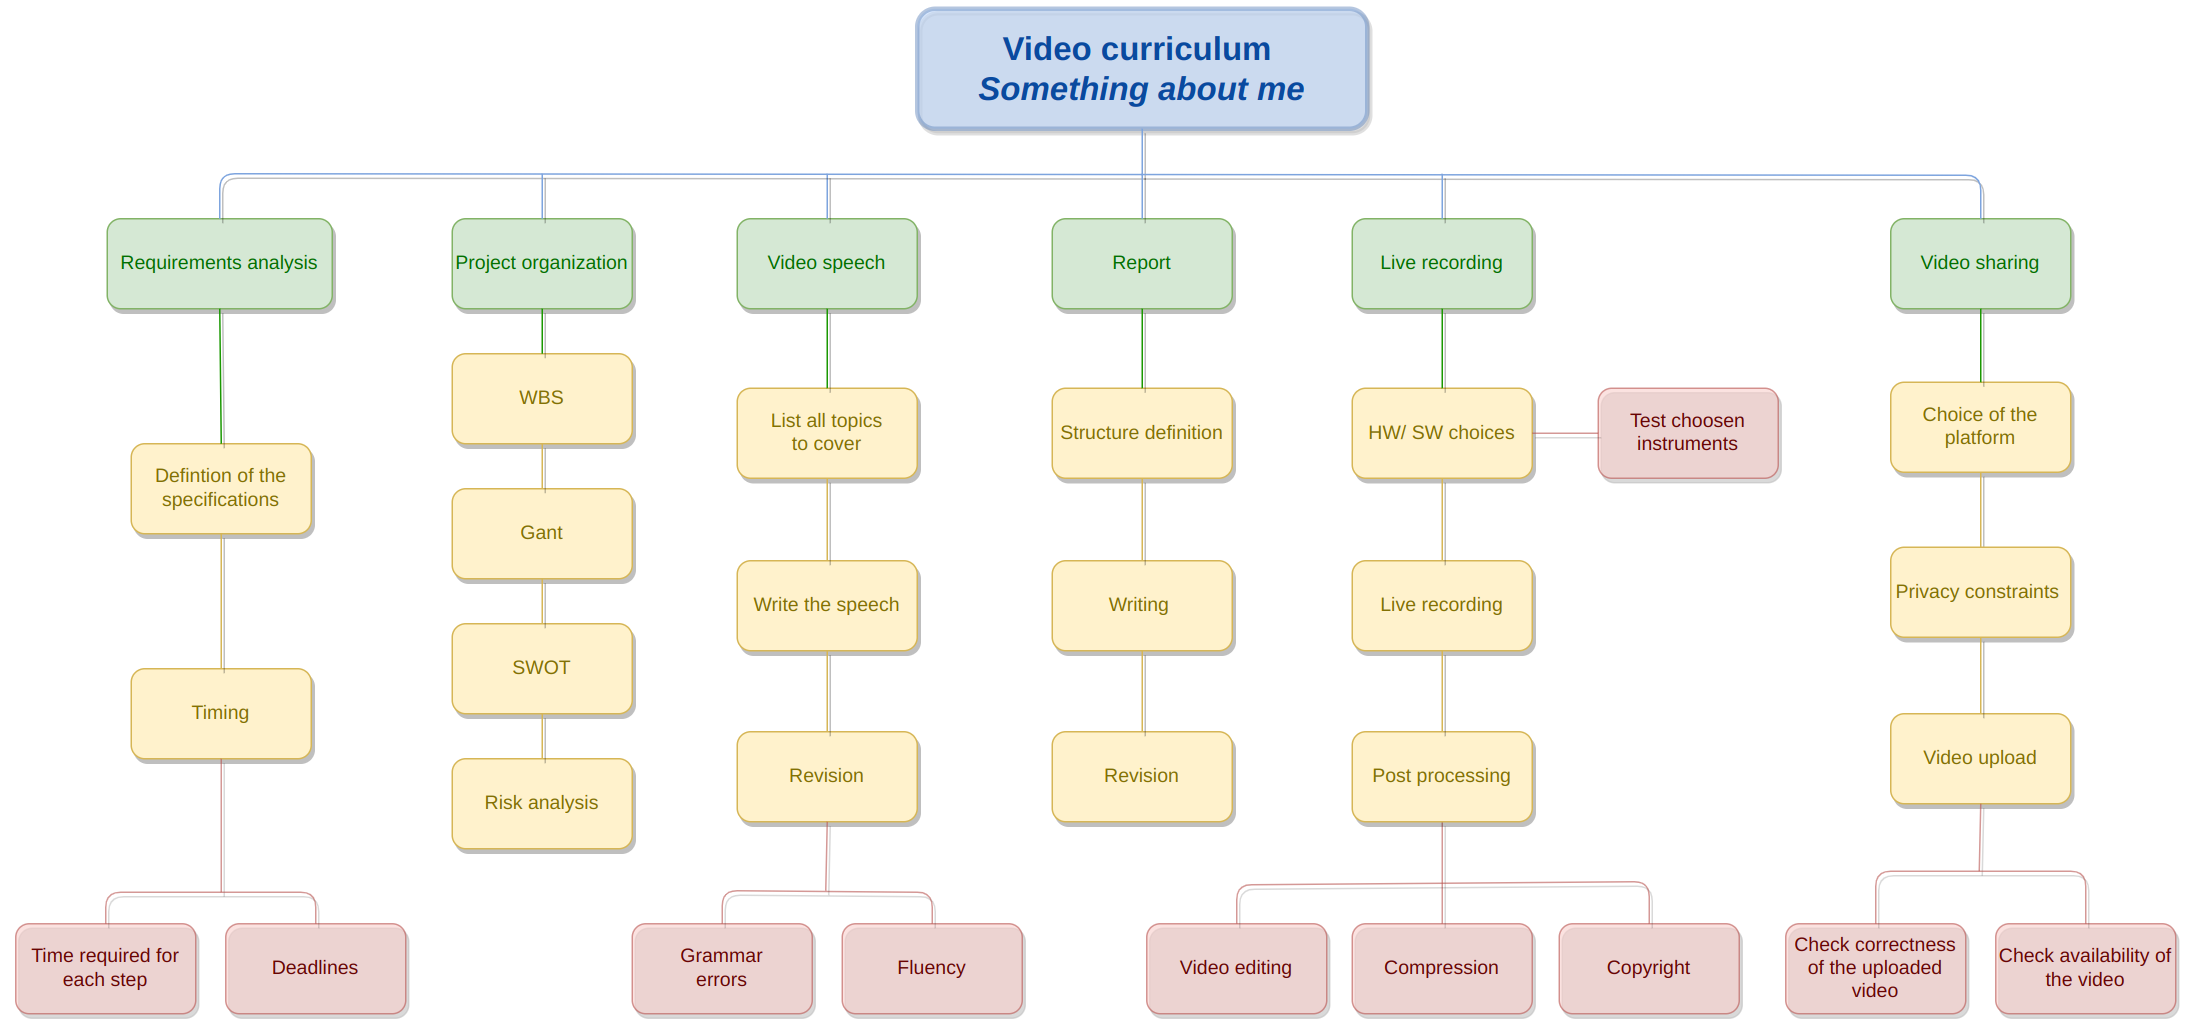
\includegraphics[width=0.9\textwidth]{images/wbs.png}
  \caption{WBS of the project}
  \label{fig-1}
\end{figure*}
\lipsum{1-2}
\section{GANTT Chart}

\begin{figure*}[h!]
  \centering
  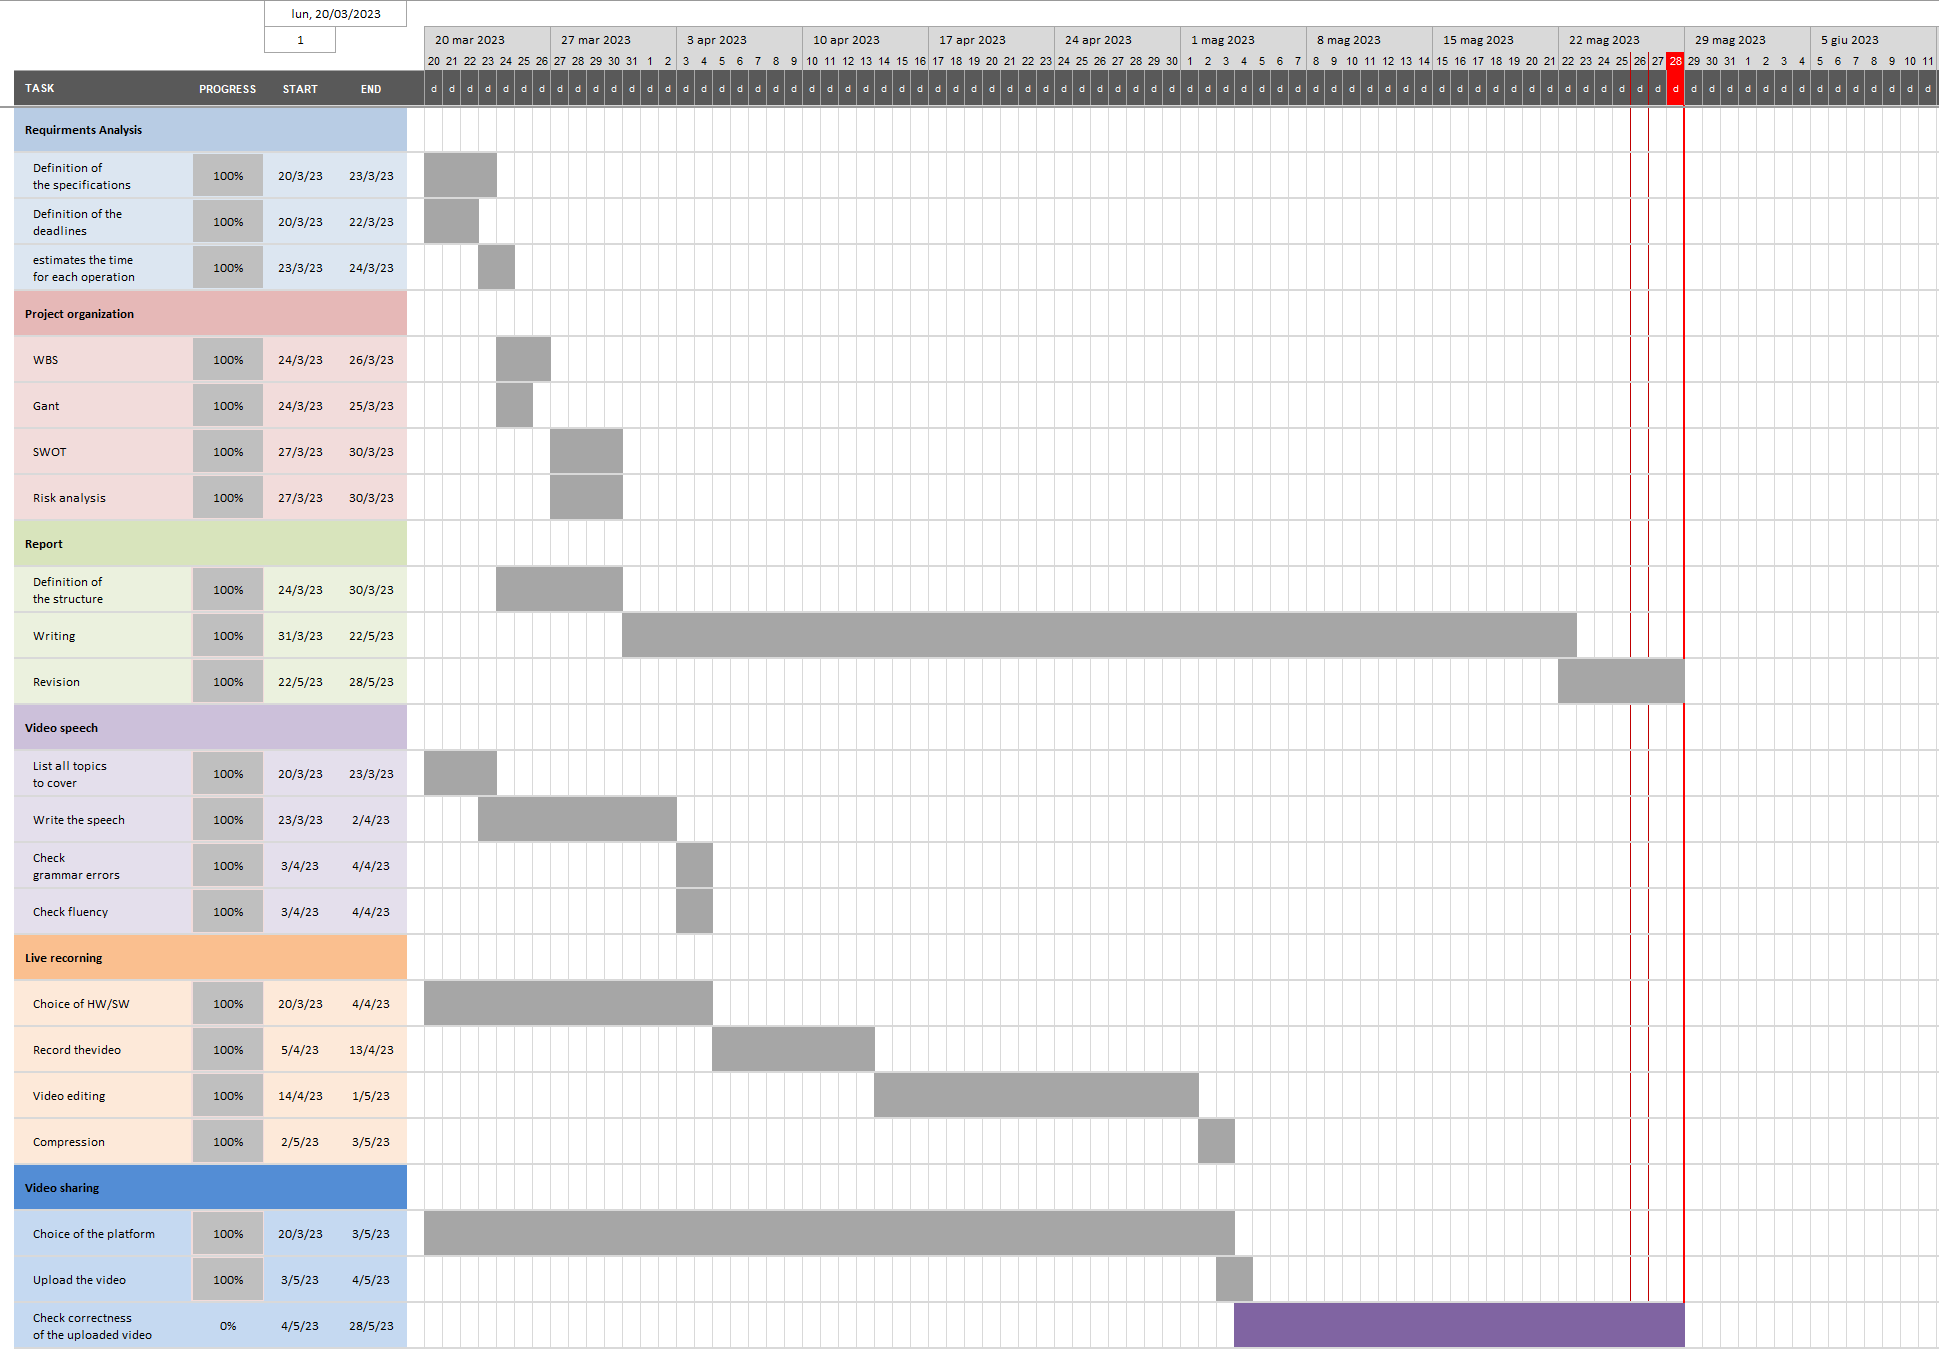
\includegraphics[width=0.9\textwidth]{images/gantt.png}
  \caption{Gantt chart}
  \label{fig-2}
\end{figure*}
\lipsum

\section{SWOT Analysis}
\section{Risk Analysis}
\section{Video creation and editing}

\section{Conclusions}

\pagestyle{OtherPage}

\end{document}